% No 'submit' option for the problems by themselves.
\documentclass[10pt]{harvardml}
% Use the 'submit' option when you submit your solutions.
%\documentclass[submit]{harvardml}

% Put in your full name and email address.
\name{Your Name}
\email{email@fas.harvard.edu}


% List any people you worked with.
\collaborators{%
  John Doe,
  Fred Doe
}

% You don't need to change these.
\course{CS281-F17}
\assignment{HW \#3}
\duedate{5pm October 20, 2017}

\usepackage{url, enumitem}
\usepackage{amsfonts}
\usepackage{listings}
\usepackage{booktabs}
\usepackage{graphicx}
\usepackage{bm}
\usepackage{tikz}
\usetikzlibrary{bayesnet}

% Some useful macros.
\newcommand{\given}{\,|\,}
\newcommand{\R}{\mathbb{R}}
\newcommand{\E}{\mathbb{E}}
\newcommand{\var}{\text{var}}
\newcommand{\cov}{\text{cov}}
\newcommand{\N}{\mathcal{N}}
\newcommand{\ep}{\varepsilon}

\theoremstyle{plain}
\newtheorem{lemma}{Lemma}

\begin{document}

\section*{Modeling Influence in a Network}

This problem considers modeling the flow of influence within a social
network using an undirected graphical model. We assume there is a new
piece of information currently gaining influence in the network. In
particular, for this example we consider a viral GIF that is being
shared among the CS281 teaching staff. For each person in the network,
we will associate a binary random variable indicating whether they are
aware of the information, e.g. RS=1 indicates that Rachit Singh has seen the GIF.
  \begin{center}
    
\includegraphics[width=4.5cm]{cat}
  \end{center}
\noindent We consider the small fixed network of (relatively unpopular) individuals with a set of connections that
  form a forest.

  \vspace{0.25cm}
  \begin{center}
\scalebox{0.8}{
  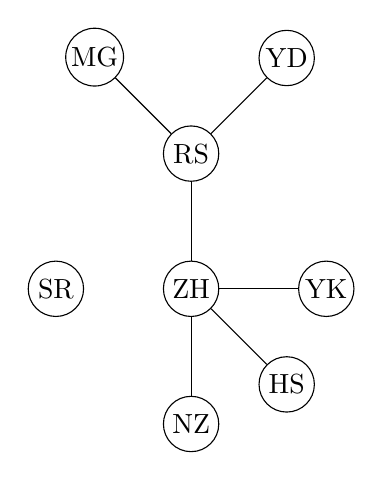
\begin{tikzpicture}
    \node(RS) [latent]{RS};
    \node(YD) [latent, above right =of RS]{YD};
    \node(MG) [latent, above left = of RS]{MG};


    \node(ZH) [latent, below =of RS]{ZH};
    \node(HS) [latent, below right =of ZH]{HS};
    \node(SR) [latent, left =of ZH]{SR};
    \node(NZ) [latent, below =of ZH]{NZ};
    \node(YK) [latent, right =of ZH]{YK};
    \draw (RS) -- (MG);
    \draw (ZH) -- (YK);
    \draw (YD) -- (RS);
    \draw (RS) -- (ZH);
    \draw (ZH) -- (NZ);
    \draw (ZH) -- (HS);
  \end{tikzpicture}
}
 \end{center}
\noindent With each person in the network we associate a unary log-potential e.g. $\theta_{\text{RS}}(0)$ and $\theta_{\text{RS}}(1)$  indicating a ``score'' for them seeing the GIF on their own.

 \begin{center}
   \begin{tabular}{ccccccccc}
     \toprule
     s & SR & YD & MG & ZH & HS & RS & NZ & YK \\
     \midrule
     $\theta_s(1)$ & 2 & -2 & -2 & -8 & -2 & 3 & -2 & 1 \\
     $\theta_s(0)$ & 0 & 0 & 0 & 0 & 0 & 0 & 0 & 0 \\
     \bottomrule
   \end{tabular}
 \end{center}

Additionally we assume a set of attractive binary log-potentials $\theta_{s - t}(1, 1) = 2$ for all connected nodes $s, t \in E$  with all other values $\theta_{s - t}(1, 0) = 0$, $\theta_{s - t}(0, 1) = 0$, $\theta_{s - t}(0, 0) = 0$  across the network.

\noindent


\begin{problem}[30pts]



  \begin{enumerate}[label=(\alph*)]

(Note: for this problem you will be deriving several properties of
    undirected graphical models and implementing these properties in
    Python/PyTorch. Before getting started it is worth getting
    familiar with the \texttt{itertools} package in Python and also
    being sure you understand how PyTorch variables work. In
    particular try writing a simple scalar function with several
    vector-valued Variables as inputs and making you understand
    what the function \texttt{.backward} does in practice.)


~


\item Implement a function for computing the global score for an
  assignment of values to the random variables, i.e. a function that
  takes in $\{0, 1\}$ values for each person and returns the
  \textit{unnormalized} value without the $A(\theta)$ term.  What is
  the score for an assignment where RS and SR are the \textit{only}
  people who have seen the GIF?

\item Implement a function for computing the log-partition function
  $A(\theta)$ using \textit{brute-force}, i.e. take in a vector
  $\theta$ and return a scalar value calculated by enumeration. What
  is its value?  Using this value compute the \textit{probability} of
  the assignment in (a)?



\vspace*{0.5cm}

 For the problems below we will be interested in computing the
  marginal probabilities for each random variable, i.e. $p(\text{SR}=1)$,
  $p(\text{RS}=1)$, etc.

\item  First, implement a function to compute $p(\text{RS}=1)$ using
  brute-force marginalization. Use the functions above to enumerate and sum all assignments with $\text{RS}=1$ .

\item Using what we know about exponential families, derive an
  expression for computing all marginals directly from the
  log-partition function $A(\theta)$. Simplify the expression.

\item Combine parts (b) and (d) to implement a method for computing
  the marginal probabilities of this model using PyTorch and
  autograd. Ensure that this gives the same value as part (c).

\item Finally compute all the marginals using exact belief propagation
  with the serial dynamic programming protocol, as described in class
  and in Murphy section 20.2.1. Use MG as the root of your graph.
  Verify that your marginals are the same as in the previous two
  calculations.

\item How do the relative values of the marginal probabilities at each
  node differ from the original log-potentials?  Explain which nodes
  values differ most and why this occurs.


\item (Optional) Implement the parallel protocol for exact BP. How does its practical speed compare to
  serial?
\end{enumerate}


\end{problem}

\newpage

\textbf{A Note on Sparse Lookups}
\vspace{0.5cm}

\noindent For the next two problems it will be beneficial to utilize sparse
matrices for computational speed. In particular our input data will consist
of sparse indicator vectors that act as lookups into a dense weight matrix. For instance, if
we say there are 500 users each associated with a vector
$\mathbb{R}^{100}$ it implies a matrix $W \in \mathbb{R}^{500 \times
  100}$. If we want a fast sparse lookup of the 1st and 10th user we can run
the following code:


\begin{verbatim}
      W = nn.Embedding(500, 100)
      x = Variable(torch.LongTensor([ [1], [10] ]))
      print(W(x))
\end{verbatim}


\noindent

This same trick can be used to greatly speed up
the calculation of bag-of-words features from the
last homework. Let's use the same example:
\begin{itemize}
\item \begin{verbatim}We like programming. We like food.\end{verbatim}
\end{itemize}
Assume that the vocabulary is
\begin{verbatim}
                 ["We", "like", "programming", "food", "CS281"]
\end{verbatim}

In last homework, we converted the above word id sequence to a vector of length of vocab size:
\begin{itemize}
\item \begin{verbatim}[2, 2, 1, 1, 0]\end{verbatim}
\end{itemize}


Instead we can convert it vector of sentence length (often much shorter):
\begin{itemize}
\item \begin{verbatim}[0, 1, 2, 0, 1, 3]\end{verbatim}
\end{itemize}

\noindent In order to calculate the same dot product between $\mathbf{x}$ and a weight vector $\mathbf{w}=[0.5,0.2,0.3,0.1,0.5]$ we can do sparse lookups and a sum:
(verify yourself that it is correct):
  \begin{verbatim}
      vocab_size = 4
      W = nn.Embedding(vocab_size, 1, padding_idx=text_field.stoi('<pad>'))
      W.weight.data = torch.Tensor([ [0.5], [0.2], [0.3], [0.1], [0.5] ])
      x = Variable(torch.LongTensor([ [0, 1, 2, 0, 1, 3] ]))
      result = torch.sum(W(x), dim=1)).squeeze()
  \end{verbatim}

This code computes the same dot-product as in HW2 but by doing 6 fast vector lookups
into $w$ and summing them together. (The \texttt{padding\_idx} part ensures
the embedding code works when there are sentences of different length by setting
a lookup of its argument to return 0. This lets you use a rectangular matrix even
with batches of different sentence lengths.) For more details, see the documentation for this module on the PyTorch website.

\newpage
%%%%%%%%%%%%%%%%%%%%%%%%%%%%%%%%%%%%%%%%%%%%%%%%%%%%%%%%%%%%%%%%%%%%%%%%%%%%%%%%
\begin{problem}[Modeling users and jokes with a latent linear model, 25pts]
In this problem, we'll use a latent linear model to jointly model the ratings
users assign to jokes. The data set we'll use is a modified and preprocessed
variant of the Jester data set (version 2) from
\url{http://eigentaste.berkeley.edu/dataset/}. The data we provide you with are user
ratings of 150 jokes. There are over 1.7M ratings with values 1, 2, 3, 4 and 5,
from about seventy thousand users. {\bf The data we give you is a modified version of the original Jester data set, see the README,
please use the files we provide and not the original ones}. The texts of the jokes are also available.
Warning: most of the jokes are bad, tasteless, or both. At best, they were
funny to late-night TV hosts in 1999-2000. Note also that some of the jokes do
not have any ratings and so can be ignored.

\textbf{Update: If you are having memory issues with this problem. Please see the note in the
readme.}

\begin{enumerate}[label=(\alph*)]
\item
Let~${r_{i,j}\in\{1,2,3,4,5\}}$ be the rating of user $i$ on joke $j$.  A latent linear model introduces a vector ${u_i\in\R^K}$ for each user and a vector~${v_j\in\R^K}$ for each joke.  Then, each rating is modeled as a noisy version of the appropriate inner product. Specifically,
\[
r_{i,j} \sim \mathcal{N}(u_i^T v_j, \sigma^2).
\]
Draw a directed graphical model with plate diagrams representing this model assuming $u_i$ and $v_j$ are random vectors.

\item Derive the log-likelihood for this model and the gradients of the log-likelihood with respect to $u_i$ and $v_j$.

\item Implement the log-likelihood calculation using PyTorch.  Compute
  the gradients using autograd and confirm that is equal to the
  manual calculation above. (Hint: Read the documentation for \texttt{nn.Embedding}
  to implement $u$ and $v$.).

\item Now set $K = 2$, $\sigma^2=1.0$ and run stochastic gradient
    descent (\texttt{optim.SGD}). We have provided a file \texttt{utils.py} to load the
    data and split it into training, validation and test sets. Note that the maximum
  likelihood estimate of $\sigma^2$ is just the mean squared error of
  your predictions on the training set. Report your MLE of $\sigma^2$.

\item Evaluate different choices of $K$ on the provided validation set. Evaluate $K = 1,
\ldots, 10$ and produce a plot that shows the root-mean-squared error on both
the training set and the validation set for each trial and for each $K$. What
seems like a good value for~$K$?

 \item We might imagine that some jokes are just better or worse than others.
We might also imagine that some users tend to have higher or lower means in
their ratings. In this case, we can introduce biases into the model so that
$r_{ij} \approx u_i^\text{T} v_j + a_i + b_j + g$, where $a_i$, $b_j$ and $g$ are user,
joke and global biases, respectively.  Change the model to incorporate these
biases and fit it again with $K=2$, learning these new biases as well. Write
down the likelihood that you are optimizing. One side-effect is that you should
be able to rank the jokes from best to worst. What are the best and worst jokes
and their respective biases?  What is the value of the global bias?

 \item Sometimes we have users or jokes that only have a few ratings. We don't
want to overfit with these and so we might want to put priors on them. What are
reasonable priors for the latent features and the biases? Modify the above directed
graphical model that shows all of these variables and their relationships.
Note that you are not required to code this new model up, just discuss
resonable priors and write the graphical model.


\end{enumerate}
\end{problem}



\section*{Ordinal Regression}

\textbf{Update: If you are running into memory issues with this problem. Please see the note in the
readme.}


We now address the problem of predicting joke ratings given the text of the
joke. The previous models assumed that the ratings where continuous real
numbers, while they are actually integers from 1 to 5. To take this into
account, we will use an ordinal regression model.
Let the rating values
be $r = 1,\ldots,R$. In the ordinal regression model the real line is
partitioned into $R$ contiguous intervals with boundaries

\begin{align}
b_1 < b_2 < \ldots < b_{R+1} = +\infty\,,
\end{align}

\noindent such that the interval $[b_r,b_{r+1})$ corresponds to the $r$-th rating value.
We will assume that $b_1 = -4$, $b_2 = -2$, $b_3 = 0$, $b_4 = 2$ and $b_5 = 4$.
Instead of directly modeling the ratings, we will be modeling them in terms of a
hidden variable $f$. We have that the rating $y$ is observed
if $f$ falls in the interval for that rating. The conditional probability of
$y$ given $f$ is then
\begin{align}
p(y = r\ |\ f) =
\left\{
    \begin{array}{ll}
        1  & \mbox{if }\quad  b_r \leq f < b_{r+1} \\
        0 & \mbox{if } \quad \mbox{otherwise}
    \end{array}
\right.
= \Theta(f - b_r) - \Theta(f-b_{r+1})\,,
\end{align}
where $\Theta(x)$ is the Heaviside step function, that is, $\Theta(x)=1$ if
$x>0$ and $\Theta(x)=0$ otherwise.


Notably there are many possible values that of $f$ that can lead to
the same rating.  This uncertainty about the exact value of $f$ can be
modeled by adding \textit{additive Gaussian noise} to a noise free
prediction. Let $\sigma^2$ be the variance of this noise. Then
$p(f\ |\ h) = \mathcal{N}(f|h,\sigma^2)$, where $h$ is a new latent
variable that is the noise free version of $f$.

Given some features $\mathbf{x}$ for a particular joke, we can then combine the
previous likelihood with a linear model to make predictions for the possible
rating values for the joke. In particular, we can assume that the noise-free
rating value $h$ is a linear function of $\mathbf{x}$, that is
$h(\mathbf{x})=\mathbf{w}^\text{T} \mathbf{x}$, where $\mathbf{w}$ is a vector
of regression coefficients. We will assume that the prior for $\mathbf{w}$ is
$p(\mathbf{w})=\mathcal{N}(\bm 0, \mathbf{I})$.





\vspace{0.5cm }
\noindent
Computational Note for this Problem: \textbf{You will need the following numerical trick,
which is implemented as \textit{log\_difference} in utils.}

If $a > b $ but $a-b$ is close to 0, you can compute $\log(a-b)$
instead as:

\[\log(1 - \exp(\log b - \log a))+\log a \]

\noindent Because $a$ is always larger than $b$ we have that $\exp(\log a- \log b )$
is always smaller than 1 and larger than 0. Therefore,
$\log(1 - \exp(b - a))$ is always well defined.

% An alternative way to compute $\log(a-b)$ is by computing $\log((1-b)-(1-a))$:

% \[\log(1 - \exp(\log (1-a) - \log (1-b)))+\log (1-b) \]

% If $a\to b, b\to 0$, then the first method is more numerically stable; if $a\to b, b\to 1$, then the
% second method is more numerically stable. Therefore, a more numerically stable way of calculating $\log(a-b)$ is:

% \[\text{torch.max}\left(\log(1-\exp(\log b-\log a))+\log a, \log(1 - \exp(\log (1-a) - \log (1-b)))+\log (1-b) \right)\]


\begin{problem}[Ordinal linear regression 25pts]
\begin{enumerate}
\vspace{-0.1cm}
~

\item Draw the directed graphical model for applying this model to one data point.

\item Compute the form of  $p(y\ |\ h)$ in the ordinal regression model. Explain
  how this would differ from a model with no additive noise term.

\vspace{-0.1cm}


\item Give the equation for the mean of the predictive distribution in the ordinal regression model.
How would is this term affected by $\sigma^2$ (include a diagram).

\vspace{-0.1cm}
\item Implement a function to compute the log-posterior distribution of the ordinal
regression model up to a normalization constant. Use autograd to compute
the gradients of the previous function with respect to $\mathbf{w}$ and
$\sigma^2$. Finds the MAP solution for $\mathbf{w}$ and
  $\sigma^2$ in the ordinal regression model given the available
  training data using SGD. Report the average RMSE on the provided test set. We have provided some helper
  functions in \texttt{utils.py}.



\vspace{-0.1cm}
\item Modify the previous model to have a Gaussian likelihood, that
  is, $p(y=r\ |\ h)=\mathcal{N}(r\ | \ h,\sigma^2)$. Report the resulting
  average test RMSE of the new model. Does performance increase or
  decrease? Why?  \vspace{-0.1cm}

\vspace{-0.1cm}
\item Consider a variant of this model with
  $\sigma^2(\mathbf{x}) = \mathbf{w_{\sigma}}^\top \mathbf{x}$. How would this
  model differ? (Optional) Implement this model.

\vspace{-0.1cm}
\item How does the performance of the models analyzed in this problem
  compare to the performance of the model from Problem 2? Which model
  performs best? Why?

\end{enumerate}
\end{problem}

\end{document}
